\documentclass[conference]{IEEEtran}
\IEEEoverridecommandlockouts
\usepackage[utf8]{inputenc}
\usepackage[T1]{fontenc}
\usepackage[spanish,es-tabla,es-nodecimaldot]{babel}
\usepackage{cite}
\usepackage{amsmath,amssymb}
\usepackage{graphicx}
\usepackage{booktabs}
\usepackage{url}
\graphicspath{{figuras/}}
% IEEE usa "Fig." en los pies de figura y "Palabras clave" en español
\addto\captionsspanish{\renewcommand{\figurename}{Fig.}}
\renewcommand{\IEEEkeywordsname}{Palabras clave}
\newcommand{\cizq}{c_u^{\mathrm{izq}}}
\newcommand{\cder}{c_u^{\mathrm{der}}}

\begin{document}

\title{Tomates 3D: detección y localización tridimensional de tomates mediante segmentación de instancias YOLO11 y visión estéreo}

\author{
\IEEEauthorblockN{Lucas García}
\IEEEauthorblockA{\textit{Facultad de Ingeniería} \\
Universidad Nacional de Asunción\\
San Lorenzo, Paraguay \\
lucas.garcia@fiuna.edu.py}
\and
\IEEEauthorblockN{Danis González}
\IEEEauthorblockA{\textit{Facultad de Ingeniería} \\
Universidad Nacional de Asunción\\
San Lorenzo, Paraguay \\
danis.gonzalez@fiuna.edu.py}
}

\maketitle

\begin{abstract}
Este trabajo presenta un sistema de visión artificial que detecta tomates cosechables y estima su posición tridimensional con dos cámaras web de bajo costo, como paso previo a la cosecha robótica. Se entrenaron tres modelos de segmentación de instancias YOLO11-seg sobre el dataset Laboro Tomato, con una búsqueda en grilla secuencial sobre la tasa de aprendizaje y el tamaño de la red, y se los comparó con un detector clásico basado en color HSV y watershed. A partir de las máscaras se generan tres características por fruto (centroide, disparidad y diámetro equivalente), con las que se triangula la posición $(X,Y,Z)$ tras una calibración estéreo por el método de Zhang. El mejor modelo (YOLO11m-seg, tasa de aprendizaje 0,0005) obtuvo en test un mAP50-95 de máscara de 0,766, un recall de 0,869 y un F1 de 0,891. En una prueba real con un tomate a 47~cm, el sistema midió $47{,}77\pm0{,}02$~cm, un error sistemático de 8~mm atribuible a la posición del centro óptico.
\end{abstract}

\begin{IEEEkeywords}
YOLO11, segmentación de instancias, visión estéreo, cosecha robótica, tomate, profundidad
\end{IEEEkeywords}

% =====================================================================
\section{Introducción}
La cosecha selectiva de cultivos de alto valor, como el tomate, sigue siendo una de las tareas agrícolas más intensivas en mano de obra: los frutos maduran de forma heterogénea y solo deben recogerse los que están listos. La escasez de trabajadores rurales y el aumento de la demanda de alimentos han impulsado el desarrollo de robots de cosecha selectiva, cuyo principal obstáculo es la percepción en un entorno con alta variabilidad, oclusiones por hojas y tallos e iluminación cambiante~\cite{kootstra2021,rajendran2024}.

Un robot cosechador necesita resolver dos problemas distintos: \emph{reconocer} el fruto en la imagen y \emph{localizarlo} en el espacio para planificar el movimiento de la pinza. Para el primero, las redes neuronales convolucionales desplazaron a los métodos clásicos basados en umbrales de color. Los detectores de una etapa de la familia YOLO~\cite{redmon2016} ofrecen inferencia en tiempo real, mientras que los modelos de segmentación de instancias como Mask R-CNN~\cite{he2017} entregan además la máscara de cada fruto, con un costo de cómputo mayor. Para el segundo problema, la visión estéreo binocular es una alternativa de bajo costo a los sensores de profundidad activos: con dos cámaras separadas una distancia conocida, el desplazamiento horizontal de un punto entre ambas imágenes (disparidad) determina su distancia por triangulación.

Trabajos recientes combinan ambas ideas. Zheng \emph{et al.}~\cite{zheng2023} segmentan tomates de invernadero con una versión liviana de YOLOv5n-seg, recortan con la máscara la nube de puntos obtenida por RAFT-Stereo y ajustan una esfera, con un error medio de localización de hasta $\pm5$~mm. Zhao \emph{et al.}~\cite{zhao2025} integran YOLOv5 con el algoritmo de correspondencia semiglobal SGBM~\cite{hirschmuller2008} y reportan una precisión de detección de 94,1~\% con errores de distancia de 3 a 5~mm. Ambos confirman que la máscara o la caja del detector permiten aislar los píxeles del fruto antes de medir su profundidad.

Este trabajo propone \emph{Tomates 3D}, un sistema completo que (i) segmenta tomates maduros y semimaduros con YOLO11-seg~\cite{yolo11}, la versión más reciente de Ultralytics; (ii) estima la profundidad a partir de la disparidad entre los centroides de las máscaras izquierda y derecha, en lugar de depender de la textura de la piel del fruto, que es lisa y degrada la correspondencia densa; y (iii) expone todo el flujo, incluida la calibración, en una interfaz web con modo en vivo. Además, se compara el enfoque de aprendizaje profundo con un detector clásico sin entrenamiento para responder si el problema realmente requiere una red neuronal.

% =====================================================================
\section{Dataset}
Se utilizó Laboro Tomato~\cite{laboro}, un conjunto público de fotografías de tomates tomadas en invernadero con teléfono móvil ($3024\times4032$~px) y anotadas en formato COCO con un polígono por fruto. Contiene 643 imágenes de entrenamiento y 161 de test con seis categorías: tomate grande (\texttt{b\_}) y cherry (\texttt{l\_}), cada uno verde, semimaduro o maduro. Se eligió porque provee máscaras de segmentación, no solo cajas, y porque sus escenas reales incluyen oclusión por hojas y racimos.

\subsection{Definición de la clase y balanceo}
El problema se planteó con una sola clase, \emph{tomate cosechable} = maduro $\cup$ semimaduro; los 6450 frutos verdes no se convierten y quedan como fondo. En una primera versión (v1) solo los maduros formaban la clase, y el modelo aprendió la regla ``naranja = ignorar''. Bajo luz cálida de interior (2700--3000~K) un tomate rojo se registra con un tono desplazado hacia el naranja y dejaba de detectarse. Al unir ambas categorías (versión v2), el límite de decisión se desplaza hacia el verde, que la iluminación no confunde, y el número de ejemplos casi se duplica.

\begin{table}[t]
\caption{Partición del dataset Laboro Tomato tras el filtrado}
\label{tab:particion}
\centering
\begin{tabular}{lrrrr}
\toprule
Partición & Imágenes & Negativas & Tomates & Tom./img$^{\dagger}$ \\
\midrule
Entrenamiento & 547 & 75 & 2325 & 4,9 \\
Validación & 96 & 17 & 322 & 4,1 \\
Test & 161 & 25 & 680 & 5,0 \\
\midrule
Total & 804 & 117 & 3327 & 4,8 \\
\bottomrule
\multicolumn{5}{l}{\footnotesize $^{\dagger}$Tomates por imagen con al menos un tomate de la clase.}
\end{tabular}
\end{table}

\begin{figure}[t]
\centering
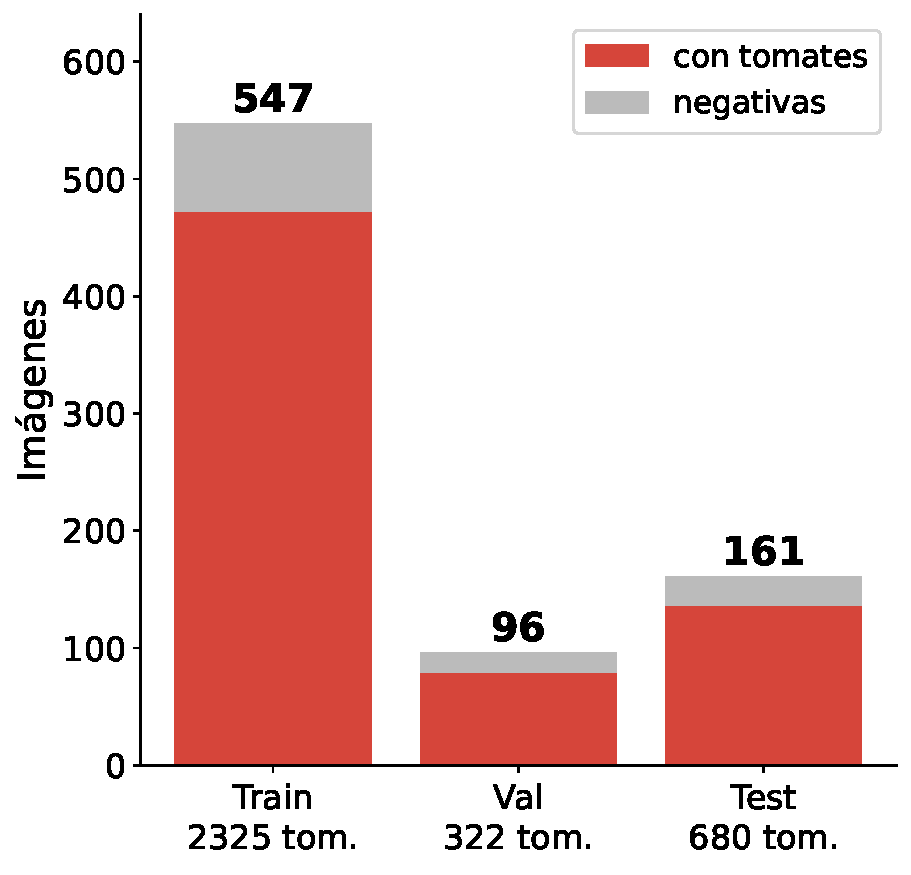
\includegraphics[width=0.82\columnwidth]{fig1_particion.pdf}
\caption{Imágenes por partición (rojo: con tomates; gris: negativas) y número de instancias de la clase en cada una.}
\label{fig:particion}
\end{figure}

En detección de una sola clase el desbalance relevante es objeto frente a fondo, que YOLO gestiona con su asignador de etiquetas y pérdidas sigmoides por posición~\cite{feng2021}. Los 6450 verdes (relación 1\,:\,1,9 con la clase) actúan como negativos difíciles: comparten forma y textura y obligan a la red a usar el color. Además se conservaron 117 imágenes sin tomates de la clase, con etiqueta vacía, para reducir falsos positivos. No se aplicó sobremuestreo ni pesos por clase.

\subsection{Preprocesamiento y partición}
Cada instancia se convirtió al formato YOLO-seg (\texttt{clase x1 y1 ...}) con coordenadas normalizadas en $[0,1]$; si una anotación tenía varios polígonos se conservó el de mayor área. Las imágenes se redujeron a 1280~px de lado mayor. El test original de Laboro se mantuvo intacto y nunca participó de una decisión; el entrenamiento original se dividió al azar 85/15 en entrenamiento y validación con semilla fija. La Tabla~\ref{tab:particion} y la Fig.~\ref{fig:particion} resumen la partición; la proporción de imágenes negativas es similar en los tres subconjuntos (14, 18 y 16~\%).

% =====================================================================
\section{Metodología}
La Fig.~\ref{fig:arquitectura} muestra el flujo completo. Dos cámaras Logitech C270 ($1280\times720$~px) separadas 8,1~cm capturan un par de imágenes; el navegador lo envía por WebSocket a una API FastAPI en Google Colab (GPU T4), que lo rectifica, produce la máscara de cada tomate en ambas vistas con un modelo de segmentación y, a partir de ellas, genera las características que permiten triangular su posición.

\begin{figure}[t]
\centering
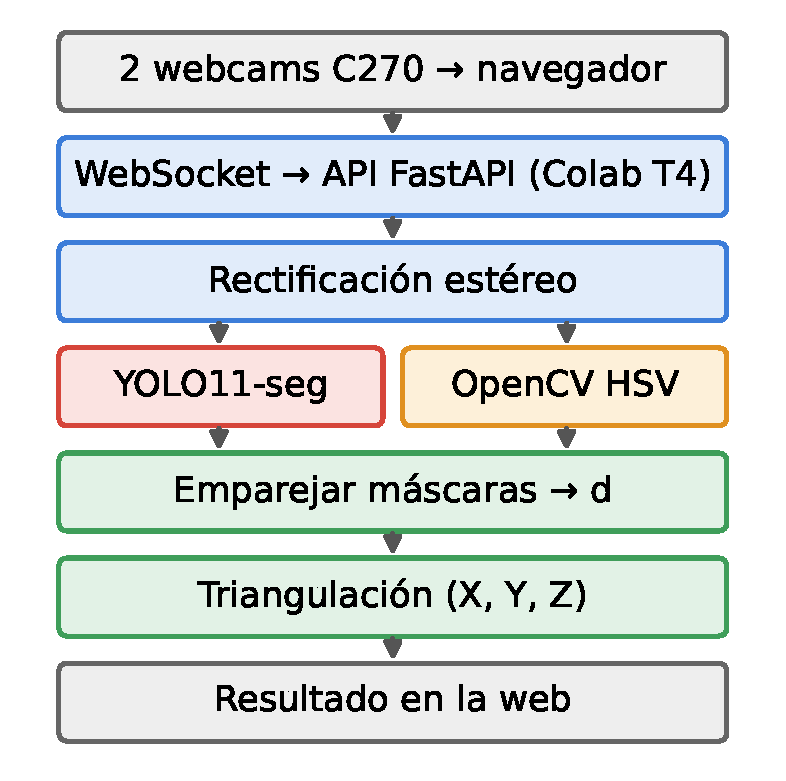
\includegraphics[width=0.82\columnwidth]{fig2_arquitectura.pdf}
\caption{Arquitectura del sistema: captura en el navegador, API en Google Colab, rectificación, segmentación con YOLO11-seg u OpenCV, emparejamiento de máscaras y triangulación de $(X,Y,Z)$.}
\label{fig:arquitectura}
\end{figure}

\begin{table}[t]
\caption{Resultados de la calibración estéreo}
\label{tab:calib}
\centering
\begin{tabular}{ll}
\toprule
Parámetro & Valor \\
\midrule
Error RMS de reproyección & 0,368 px \\
Línea base $B$ (calculada / regla) & 8,14 cm / $\approx$8 cm \\
Focal rectificada $f$ & 1605,9 px \\
Rotación entre cámaras & $\approx$0,9$^\circ$ \\
Resolución & $1280\times720$ px \\
\bottomrule
\end{tabular}
\end{table}

\subsection{Calibración estéreo y rectificación}
Se usa el modelo de cámara estenopeica, en el que un punto $(X,Y,Z)$ se proyecta en el píxel $u=f_xX/Z+c_x$, $v=f_yY/Z+c_y$, con distorsión radial y tangencial de Brown-Conrady. Los parámetros intrínsecos se estiman por el método de Zhang~\cite{zhang2000} a partir de 15--25 vistas de un tablero de $9\times6$ esquinas internas, y la rotación $R$ y traslación $T$ entre cámaras se obtienen minimizando el error de reproyección conjunto. La rectificación de Bouguet~\cite{bradski2008} rota virtualmente ambas cámaras para que las líneas epipolares queden horizontales: el correspondiente de $(u,v)$ está en $(u-d,v)$. Toda la calibración se realiza desde la interfaz web; los resultados se muestran en la Tabla~\ref{tab:calib}.

\subsection{Features generados}
Para cada máscara binaria $M$ de un tomate, con $N$ píxeles en posiciones $(u_i,v_i)$, se calculan tres características geométricas.

\subsubsection{Centroide}
Es el punto medio de la silueta y, para un fruto aproximadamente esférico, la proyección de su centro:
\begin{equation}
c_u=\frac{1}{N}\sum_{i=1}^{N}u_i,\qquad c_v=\frac{1}{N}\sum_{i=1}^{N}v_i .
\end{equation}
Al promediar miles de píxeles, un error de un píxel en el contorno desplaza el centroide solo una fracción de píxel.

\subsubsection{Disparidad}
Cada máscara izquierda se empareja con la máscara derecha del mismo fruto, y la disparidad del centro es
\begin{equation}
d=\cizq-\cder .
\end{equation}
Un par es candidato si $|c_v^{\mathrm{izq}}-c_v^{\mathrm{der}}|\le\max(12\,\mathrm{px},\,0{,}25h)$, donde $h$ es la altura de la caja; si $0{,}5<d<1{,}2\,d_{\max}$; y si la relación de áreas está entre 0,6 y 1,6. Se descartan las máscaras que tocan el borde lateral, cuyo centroide está sesgado. Esta característica no depende de la textura de la piel, a diferencia de la correspondencia por bloques.

\subsubsection{Diámetro equivalente}
Estima el tamaño físico del fruto a partir del área de la máscara $A=N$ (en píxeles):
\begin{equation}
D=2\sqrt{A/\pi}\,\frac{Z}{f}.
\end{equation}

Con estas características, la posición del centro del tomate respecto de la cámara izquierda rectificada se obtiene por triangulación (Fig.~\ref{fig:triangulacion}):
\begin{equation}
Z=\frac{fB}{d},\qquad X=\frac{(c_u-c_x)Z}{f},\qquad Y=\frac{(c_v-c_y)Z}{f}.
\label{eq:triang}
\end{equation}
Con $f=1605{,}9$~px y $B=0{,}08139$~m, $fB=130{,}7$~px$\cdot$m; un tomate a 47~cm produce $d\approx278$~px. Cuando no hay pareja de máscaras, se usa como respaldo el mapa de disparidad SGBM~\cite{hirschmuller2008} dentro de la máscara erosionada (mediana entre los percentiles 20 y 80) más un radio estimado.

\begin{figure}[t]
\centering
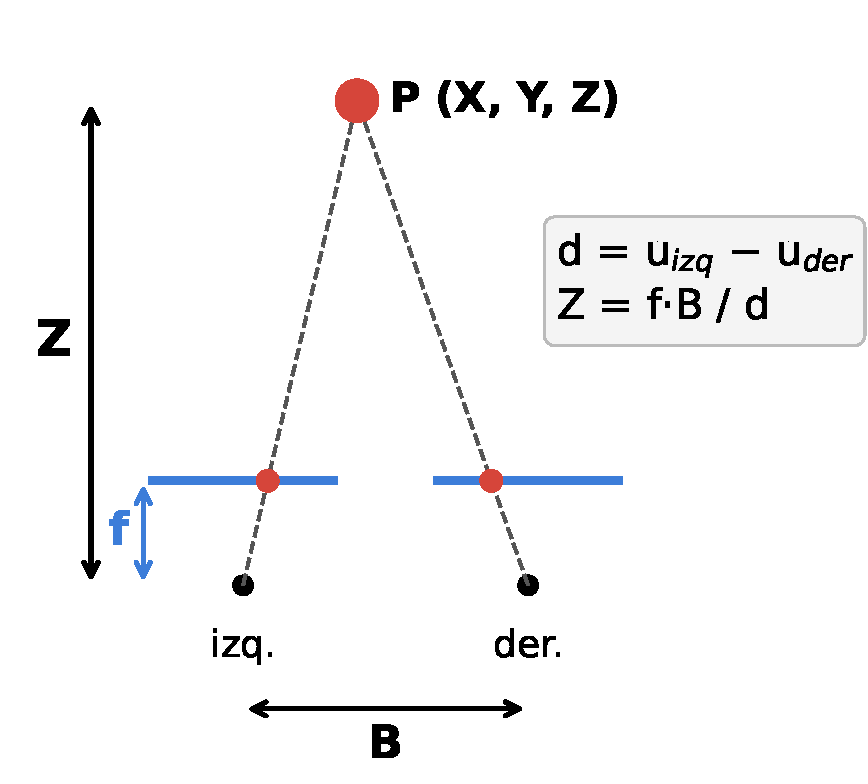
\includegraphics[width=0.78\columnwidth]{fig3_triangulacion.pdf}
\caption{Vista superior de la triangulación estéreo: el punto $P$ se proyecta en $u_{\mathrm{izq}}$ y $u_{\mathrm{der}}$; su diferencia es la disparidad $d$.}
\label{fig:triangulacion}
\end{figure}

\subsection{Modelo base: YOLO11-seg}
YOLO11-seg~\cite{yolo11} es un detector de una etapa que predice en paralelo cajas, clases y máscaras. Su \emph{backbone} reduce la imagen 32 veces con convoluciones $3\times3$ de paso 2 y bloques CSP (C3k2), y termina en un módulo SPPF de contexto multiescala y un bloque de autoatención C2PSA. El \emph{neck} FPN+PAN fusiona rasgos de tres escalas ($80\times80$, $40\times40$ y $20\times20$), con 8400 posiciones candidatas por imagen. En cada posición, la cabeza desacoplada predice la caja sin anclas mediante \emph{Distribution Focal Loss}~\cite{li2020}, la confianza de la clase y 32 coeficientes; una proto-red genera 32 prototipos de $160\times160$ y la máscara de cada instancia se arma como en YOLACT~\cite{bolya2019}:
\begin{equation}
\hat{M}=\sigma\!\left(\sum_{k=1}^{32}a_kP_k\right).
\end{equation}
Durante el entrenamiento se minimiza la suma ponderada de las pérdidas de caja (CIoU, peso 7,5), DFL (1,5), clasificación (BCE, 0,5) y máscara (BCE por píxel), con asignación de objetivos \emph{task-aligned}~\cite{feng2021}. Se partió de pesos preentrenados en COCO~\cite{lin2014}: se transfirieron 555 de 561 tensores en el modelo $s$ y 705 de 711 en el $m$; solo se reinicializan los que dependen del número de clases ($80\to1$).

\subsection{Método de comparación: detector clásico OpenCV}
Como referencia sin aprendizaje se implementó un detector de cinco etapas (Fig.~\ref{fig:opencv}): umbral de rojo en HSV ($H\in[0,8]\cup[172,180]$, $S\ge150$, $V\ge100$), morfología (cierre de 35~px, apertura de 5~px y cierre de 11~px) para tapar reflejos, transformada de distancia suavizada, máximos locales separados al menos 45~px como semillas y watershed~\cite{bradski2008} para separar frutos que se tocan. La confianza se define como la redondez (área del contorno / área del círculo mínimo que lo encierra). El detector comparte con YOLO la rectificación, el emparejamiento y la triangulación, de modo que solo cambia la etapa de reconocimiento.

\begin{figure}[t]
\centering
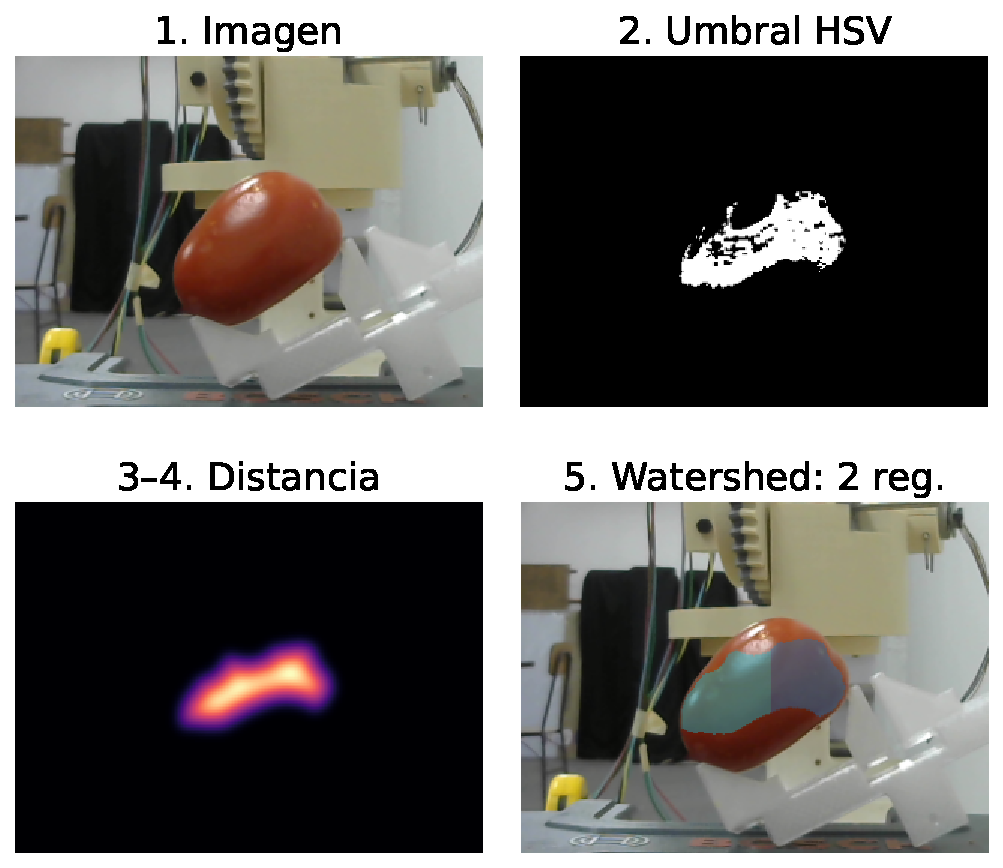
\includegraphics[width=0.82\columnwidth]{fig4_opencv_pasos.pdf}
\caption{Etapas del detector clásico sobre la captura real (recorte alrededor del tomate): imagen, umbral HSV, transformada de distancia suavizada y watershed. El fruto alargado presenta dos máximos y queda dividido en dos regiones.}
\label{fig:opencv}
\end{figure}

\subsection{Optimización de hiperparámetros}
Se aplicó una búsqueda en grilla secuencial sobre los dos hiperparámetros con mayor efecto esperado: la tasa de aprendizaje inicial $\mathrm{lr}_0\in\{0{,}002;\;0{,}0005\}$ y el tamaño de la red $\in\{s,m\}$, variando una sola dimensión por vez. M1 y M2 comparten arquitectura (YOLO11s-seg) y solo difieren en $\mathrm{lr}_0$; el valor 0,002 es el que Ultralytics elige automáticamente para este caso. El mejor $\mathrm{lr}_0$, seleccionado por el mAP50-95 de máscara en validación, se usó en M3 (YOLO11m-seg), que solo cambia el tamaño. La combinación $m$ con $\mathrm{lr}_0=0{,}002$ no se ejecutó porque ese valor ya había sido descartado en el modelo pequeño. Además, las tres configuraciones se entrenaron con las dos definiciones de la clase (v1 y v2). Con un costo de 0,5--0,9~h de GPU por configuración, se prefirió este diseño controlado frente a una búsqueda bayesiana (Optuna), que habría requerido decenas de entrenamientos.

El resto de los hiperparámetros se mantuvo fijo (Tabla~\ref{tab:fijos}) para que cada diferencia sea atribuible a la variable estudiada. Se usó AdamW~\cite{loshchilov2019}, que aplica el \emph{weight decay} desacoplado del gradiente y converge rápido con pocos datos.

\begin{table}[t]
\caption{Hiperparámetros fijos del entrenamiento}
\label{tab:fijos}
\centering
\begin{tabular}{lp{4.6cm}}
\toprule
Parámetro & Valor \\
\midrule
Plataforma & Colab, GPU Tesla T4, AMP (FP16) \\
Pesos iniciales & COCO (transfer learning) \\
Épocas / paciencia & 100 / 25 (ninguno se detuvo) \\
Imagen / batch & 640 px / 16 (35 iter./época) \\
Optimizador & AdamW, momento 0,937 \\
Programa de lr & warm-up 3 épocas, decaimiento lineal a $0{,}01\,\mathrm{lr}_0$ \\
Weight decay & 0,0005 \\
Aumento de datos & mosaic (off últimas 10 épocas), flip, escala $\pm50$~\%, rotación $\pm10^\circ$, HSV con $h=0{,}005$ \\
Semilla & 0, determinista \\
\bottomrule
\end{tabular}
\end{table}

\subsection{Métricas de evaluación}
\emph{Segmentación.} Una predicción es verdadero positivo (TP) si su IoU con un tomate anotado supera el umbral; si no, es falso positivo (FP). Los tomates sin predicción son falsos negativos (FN). Se reportan
\begin{equation}
P=\frac{TP}{TP+FP},\quad R=\frac{TP}{TP+FN},\quad F_1=\frac{2PR}{P+R},
\end{equation}
y la precisión media AP, área bajo la curva precisión-recall interpolada en 101 puntos. mAP50 usa IoU $\ge0{,}5$ y mAP50-95 promedia el AP en diez umbrales entre 0,50 y 0,95~\cite{lin2014}. La métrica principal es el mAP50-95 de máscara, porque la forma de la máscara es lo que se usa para medir $Z$. No se reporta exactitud (\emph{accuracy}) porque en detección los verdaderos negativos no son contables.

\emph{Localización.} Se mide el error de $Z$ frente a una cinta métrica, su desviación estándar en capturas repetidas y la proporción de capturas con emparejamiento correcto. La resolución teórica en profundidad se obtiene derivando~\eqref{eq:triang}:
\begin{equation}
\Delta Z=\frac{Z^2}{fB}\,\Delta d.
\label{eq:resolucion}
\end{equation}

% =====================================================================
\section{Resultados}

\subsection{Búsqueda de hiperparámetros}
La Tabla~\ref{tab:grid} muestra el resultado de cada configuración en validación (usada para decidir) y en test (usado solo para informar). Reducir $\mathrm{lr}_0$ cuatro veces (M1$\to$M2) aumentó el recall en 2,4 puntos y el mAP50-95 en 0,6 con la misma precisión. Duplicar los parámetros (M2$\to$M3) sumó 0,7 puntos de recall, 1,3 de mAP50 y 0,7 de mAP50-95 de máscara, a cambio de 2,2 veces más parámetros y 2,7 veces más tiempo de inferencia. La Fig.~\ref{fig:hiper}(b) visualiza este impacto. El mismo orden entre configuraciones se repite en la versión v1: el lr bajo mejora el recall y el modelo $m$ obtiene el mejor mAP50-95. Las métricas de v1 y v2 no son comparables número a número, porque cada versión se evalúa con su propia definición de la clase.

\begin{table*}[t]
\caption{Búsqueda en grilla de hiperparámetros y su impacto en las métricas (máscara, salvo indicación)}
\label{tab:grid}
\centering
\footnotesize
\setlength{\tabcolsep}{3.2pt}
\begin{tabular}{llllrcccccccc}
\toprule
 & & & & & Val & \multicolumn{6}{c}{Test (161 imágenes)} & \\
\cmidrule(lr){6-6}\cmidrule(lr){7-12}
Config. & Versión & Red & $\mathrm{lr}_0$ & Parám. & mAP50-95 & P & R & F1 & mAP50 & mAP50-95 & mAP50-95 caja & ms/img (T4) \\
\midrule
M1 & v2 & YOLO11s-seg & 0,002 & 10,08 M & 0,8158 & \textbf{0,919} & 0,838 & 0,877 & 0,924 & 0,753 & 0,819 & 10,0 \\
M2 & v2 & YOLO11s-seg & 0,0005 & 10,08 M & 0,8197 & 0,916 & 0,862 & 0,888 & 0,921 & 0,759 & 0,823 & \textbf{9,5} \\
M3 & v2 & YOLO11m-seg & 0,0005 & 22,36 M & \textbf{0,8287} & 0,913 & \textbf{0,869} & \textbf{0,891} & \textbf{0,934} & \textbf{0,766} & \textbf{0,834} & 25,7 \\
\midrule
M1 & v1 & YOLO11s-seg & 0,002 & 10,08 M & 0,790 & 0,833 & 0,745 & 0,787 & 0,856 & 0,698 & 0,750 & 10,4 \\
M2 & v1 & YOLO11s-seg & 0,0005 & 10,08 M & 0,800 & 0,816 & 0,795 & 0,805 & 0,865 & 0,698 & 0,758 & 10,5 \\
M3 & v1 & YOLO11m-seg & 0,0005 & 22,36 M & 0,802 & 0,816 & 0,804 & 0,810 & 0,862 & 0,710 & 0,763 & 26,2 \\
\midrule
-- & -- & YOLO11m-seg & 0,002 & 22,36 M & \multicolumn{8}{l}{no ejecutada: $\mathrm{lr}_0=0{,}002$ ya descartado en validación con la red $s$} \\
OpenCV & -- & HSV+watershed & -- & 0 & \multicolumn{8}{l}{sin entrenamiento; evaluado solo en la prueba real (Tabla~\ref{tab:real})} \\
\bottomrule
\multicolumn{13}{l}{\footnotesize v1: clase = solo maduros; v2: clase = maduros + semimaduros. Cada versión se evalúa en test con su propia definición de la clase (680 tomates en v2).}
\end{tabular}
\end{table*}

\begin{figure*}[t]
\centering
\begin{minipage}{0.44\textwidth}\centering
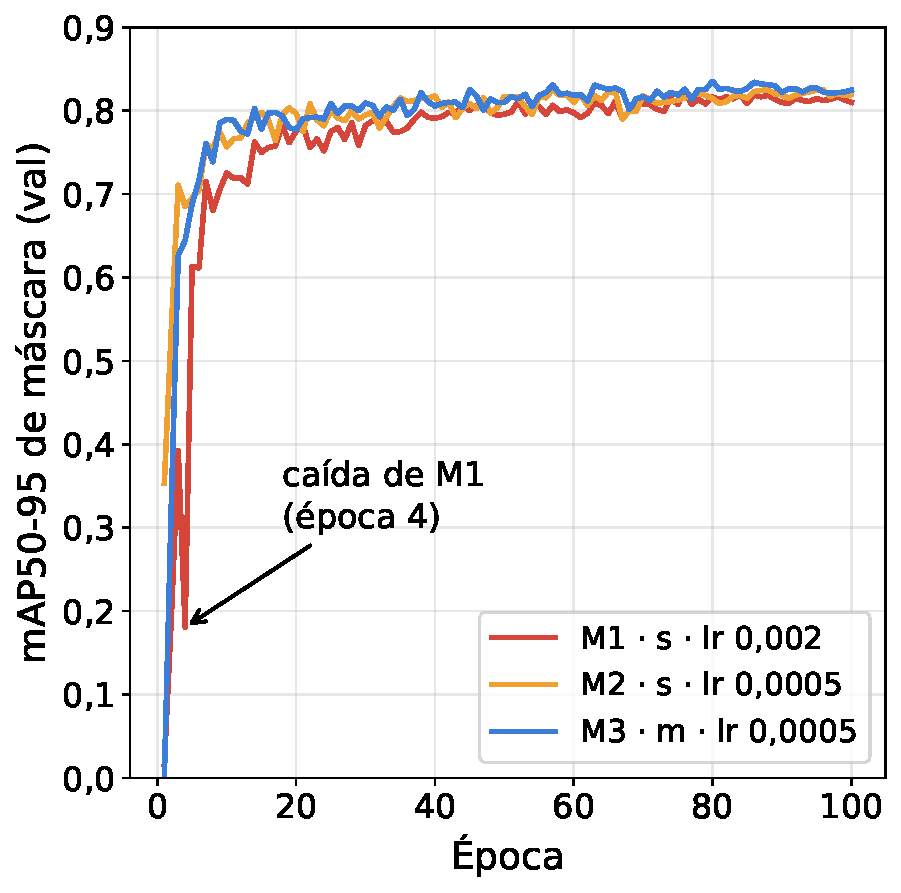
\includegraphics[width=\linewidth]{fig5a_curva.pdf}\\(a)
\end{minipage}\hfill
\begin{minipage}{0.44\textwidth}\centering
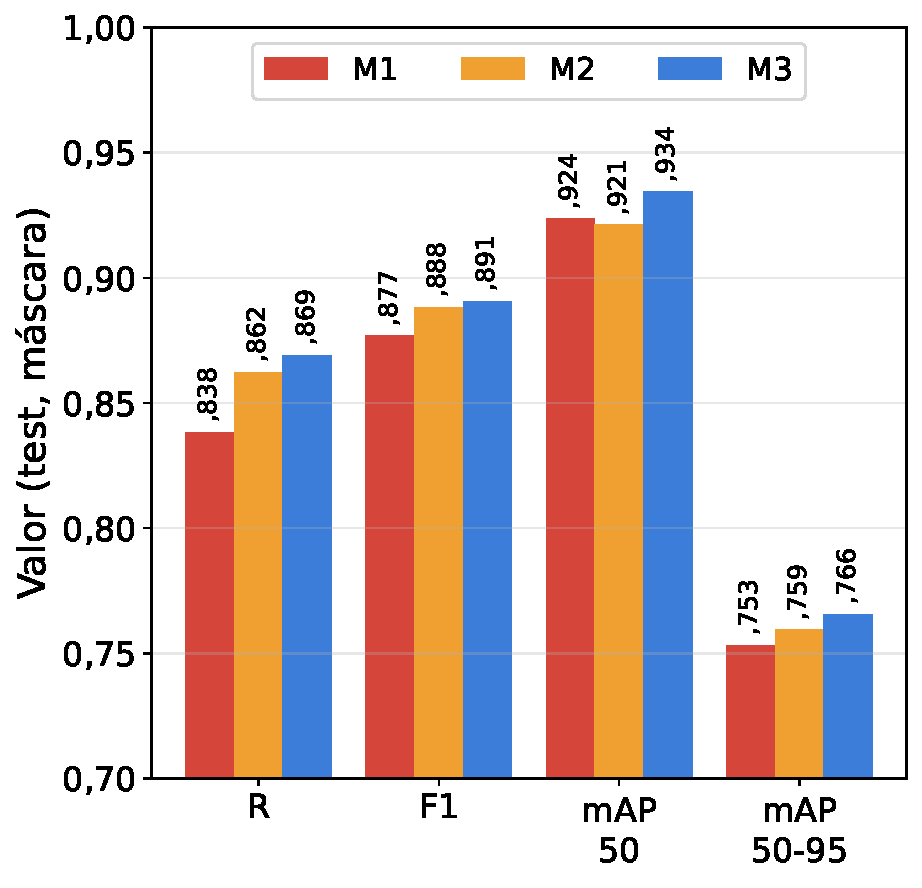
\includegraphics[width=\linewidth]{fig5b_impacto.pdf}\\(b)
\end{minipage}
\caption{(a) Curva de aprendizaje: mAP50-95 de máscara en validación por época para las tres configuraciones (v2). (b) Métricas de máscara en test de cada configuración de la búsqueda de hiperparámetros.}
\label{fig:hiper}
\end{figure*}

\subsection{Curvas de aprendizaje}
La Fig.~\ref{fig:hiper}(a) muestra que una tasa alta desestabiliza el inicio del ajuste fino: en M1 el mAP50-95 de máscara cae de 0,39 en la época~3 a 0,18 en la época~4, porque la actualización se aleja del mínimo que traían los pesos preentrenados, y se recupera cuando termina el warm-up. Con $\mathrm{lr}_0=0{,}0005$, M2 alcanza 0,71 en la época~3 sin retrocesos. Los tres modelos convergen a una meseta de 0,81--0,83 cerca de la época~40; las mejores épocas fueron 76, 57 y 80. La pérdida de segmentación de entrenamiento siguió bajando hasta el final (M2: $1{,}75\to0{,}51$) mientras la métrica de validación se mantuvo estable, lo que indica un sobreajuste leve y controlado, mitigado al conservar la mejor época.

\subsection{Matriz de confusión y errores de segmentación}
La Fig.~\ref{fig:conf}(a) presenta la matriz de confusión de M3 en test, medida con el umbral de operación del sistema (confianza $\ge0{,}35$) y un IoU de máscara $\ge0{,}5$: 613~TP, 67~FN y 120~FP sobre 680 tomates. La Tabla~\ref{tab:cm} la extiende a los tres modelos. En el umbral de máximo F1 los tres tienen una precisión de $\approx0{,}92$ (Tabla~\ref{tab:grid}); con el umbral fijo de 0,35 la precisión baja a 0,84--0,86 porque se aceptan detecciones dudosas, y M2 obtiene el mejor F1 (0,883 frente a 0,868 de M3). M3 es el mejor integrando todos los umbrales (mAP), pero no necesariamente en el punto de operación. Los modelos difieren sobre todo en los frutos difíciles (tapados por hojas, en el borde o pequeños). El mAP50-95 de máscara (0,766) es menor que el de caja (0,834) porque la máscara debe coincidir en todo el contorno, incluidas las zonas difusas; aun así, las máscaras correctas de M3 tienen un IoU mediano de 0,93.

La diferencia entre validación (0,82--0,83) y test (0,75--0,77) puede deberse en parte a que el test tiene más tomates por imagen que la validación (5,0 frente a 4,1) y a que son fotografías distintas; en cualquier caso, el test nunca se usó para decidir y es la estimación honesta del rendimiento. Se seleccionó M3, el mejor en validación, cuyo tiempo de 26~ms por imagen no limita el modo en vivo.

\begin{table}[t]
\caption{Matriz de confusión en test con el umbral de operación (confianza $\ge0{,}35$, IoU de máscara $\ge0{,}5$; 680 tomates)}
\label{tab:cm}
\centering
\begin{tabular}{lrrrccc}
\toprule
Modelo & TP & FP & FN & P & R & F1 \\
\midrule
M1 & 601 & 107 & 79 & 0,849 & 0,884 & 0,866 \\
M2 & 618 & 101 & 62 & \textbf{0,860} & \textbf{0,909} & \textbf{0,883} \\
M3 & 613 & 120 & 67 & 0,836 & 0,901 & 0,868 \\
\bottomrule
\end{tabular}
\end{table}

\begin{figure*}[t]
\centering
\begin{minipage}{0.44\textwidth}\centering
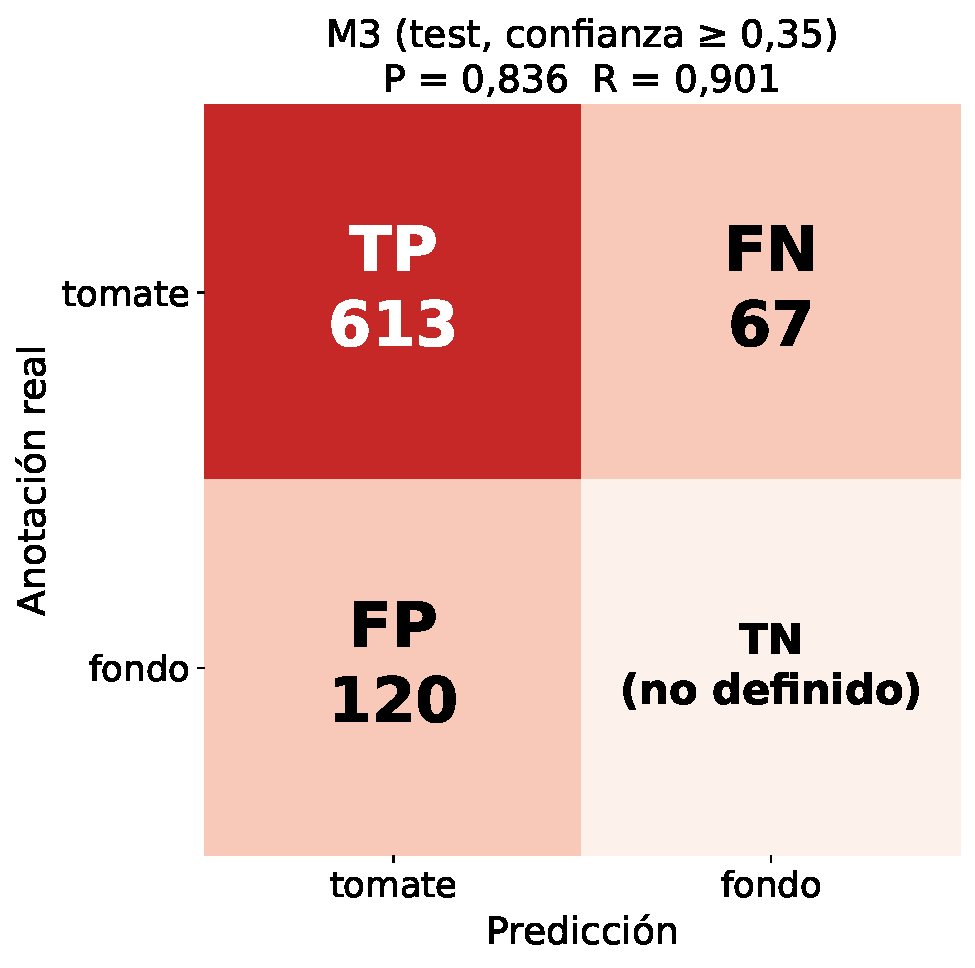
\includegraphics[width=\linewidth]{fig6a_matriz_confusion.pdf}\\(a)
\end{minipage}\hfill
\begin{minipage}{0.44\textwidth}\centering
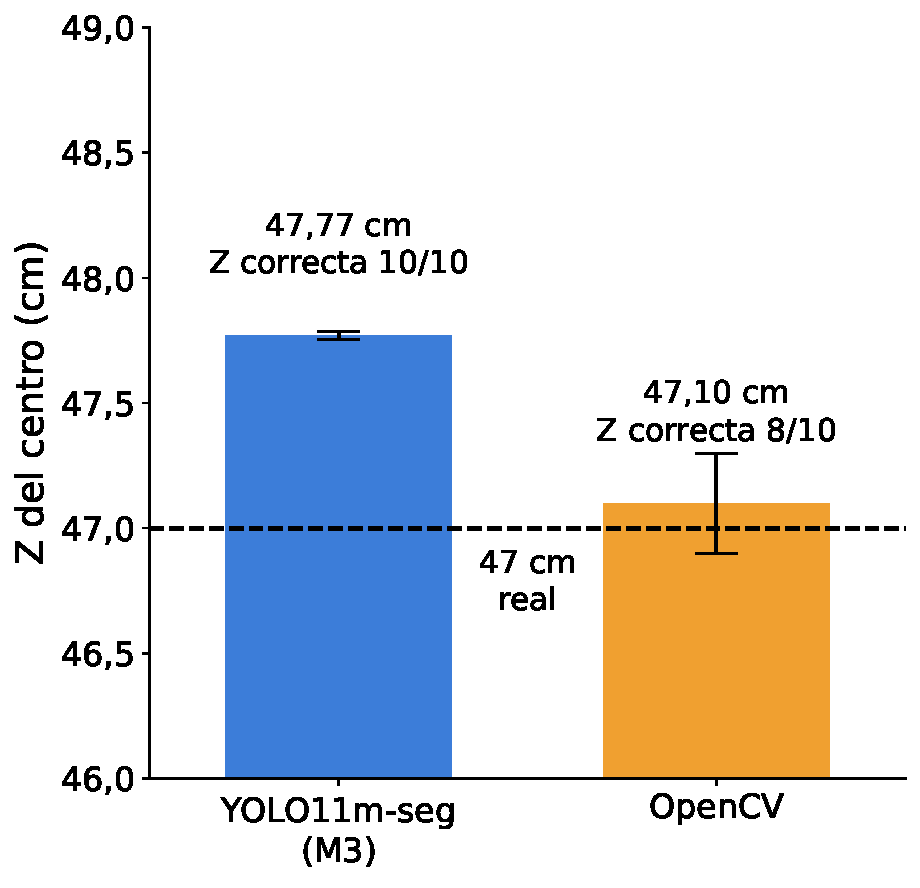
\includegraphics[width=\linewidth]{fig6b_prueba_real.pdf}\\(b)
\end{minipage}
\caption{(a) Matriz de confusión de M3 en test (680 tomates), medida con confianza $\ge0{,}35$ e IoU de máscara $\ge0{,}5$; en detección los verdaderos negativos no están definidos. (b) $Z$ medida en la prueba real (media $\pm$ desviación estándar de las capturas con emparejamiento correcto) frente a los 47~cm medidos con cinta.}
\label{fig:conf}
\end{figure*}

\subsection{Prueba real de localización}
Con un tomate sostenido por la pinza del brazo robótico a 47~cm de las cámaras (medidos con cinta al centro del fruto) se capturaron 10 pares consecutivos y se procesaron con ambos métodos (Fig.~\ref{fig:real}, Tabla~\ref{tab:real} y Fig.~\ref{fig:conf}(b)). M3 detectó el fruto completo en las 10 capturas y midió $Z=47{,}77\pm0{,}02$~cm. La dispersión de 0,2~mm indica que el error de $+0{,}8$~cm no es ruido sino un corrimiento sistemático, coincidente con el \emph{offset} de $+1{,}0$ a $+1{,}1$~cm medido antes a 52, 60 y 70~cm: la profundidad se mide desde el centro óptico, situado detrás del frente de la cámara. Las seis versiones de YOLO (M1--M3, v1 y v2) midieron entre 47,66 y 47,78~cm, por lo que la profundidad no depende del modelo elegido.

OpenCV encontró el rojo, pero dividió el fruto alargado en dos regiones en las 10 capturas y omitió la parte en sombra; en 2 de 10 pares el emparejamiento falló y produjo $Z=35$~cm. Por su parte, M3 confundió el respaldo de madera de una silla con un tomate a 3,0~m (confianza 0,94), un efecto de cambio de dominio, ya que el dataset no contiene muebles. Las tres versiones v2 cometieron este falso positivo y las v1 no: unir la clase con los semimaduros (naranjas) aumenta la sensibilidad a objetos de madera anaranjada. Como todos aparecieron a más de 2,9~m, un filtro de rango de trabajo los elimina.

\begin{table}[t]
\caption{Prueba real: 10 capturas de un tomate a 47~cm}
\label{tab:real}
\centering
\begin{tabular}{lcc}
\toprule
 & YOLO11m-seg & OpenCV \\
\midrule
Tomate detectado & 10/10 & 10/10, partido en 2 \\
$Z$ correcta & 10/10 & 8/10 \\
$Z$ centro (cm) & $47{,}77\pm0{,}02$ & $47{,}1\pm0{,}20$ \\
Error medio (cm) & $+0{,}8$ & $+0{,}1$ \\
Diámetro (cm) & 6,2 & 3,1 \\
Tiempo CPU (ms)$^{a}$ & 1066 / 1723 & 78 / 349 \\
Falsos positivos & 1 (silla a 3,0 m) & -- \\
\bottomrule
\multicolumn{3}{l}{\footnotesize $^{a}$Reconocimiento / procesamiento total del par.}
\end{tabular}
\end{table}

\begin{figure}[t]
\centering
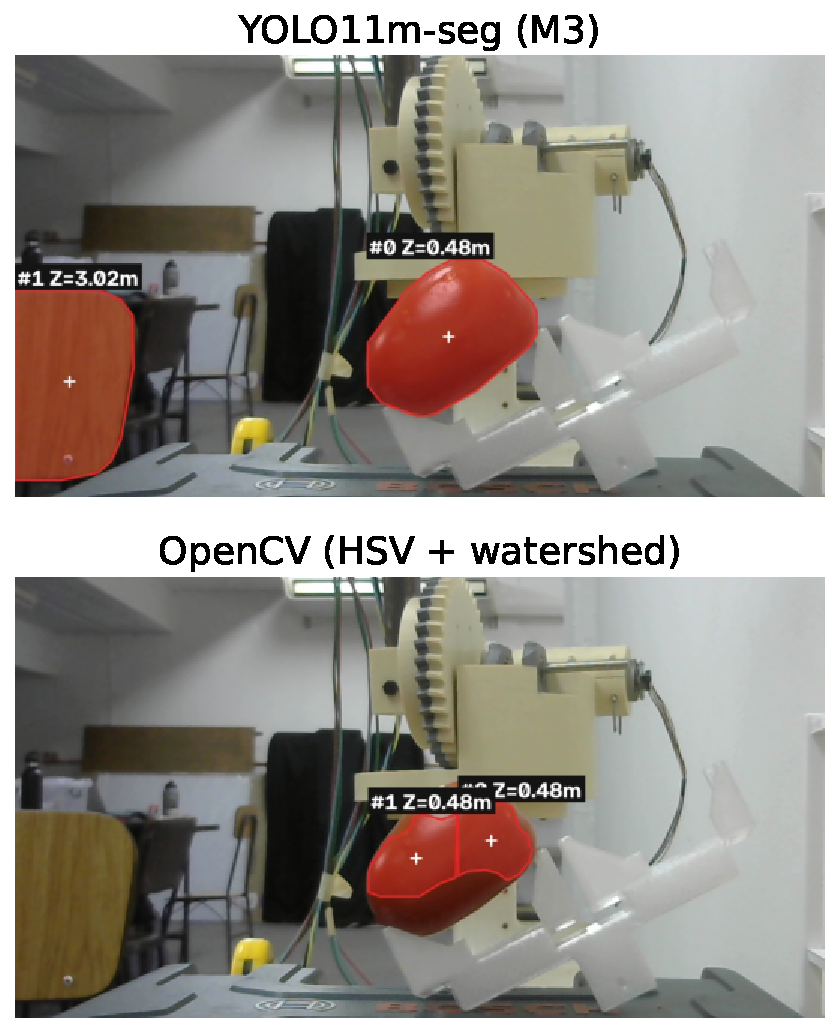
\includegraphics[width=0.85\columnwidth]{fig7_comparacion_real.pdf}
\caption{Misma captura de la prueba real (imagen izquierda rectificada) procesada con YOLO11m-seg (arriba) y OpenCV (abajo). YOLO segmenta el fruto completo (\#0, $Z=0{,}48$~m) y comete un falso positivo lejano (\#1, $Z=3{,}02$~m); OpenCV lo divide en dos.}
\label{fig:real}
\end{figure}

El error medio menor de OpenCV es engañoso: corresponde al centroide de un fragmento del fruto y no a su centro, como confirma el diámetro de 3,1~cm frente a los 6,2~cm de M3. En la misma prueba, SGBM sobre la piel lisa del tomate asignó a la ``superficie'' 47,73~cm, prácticamente el centro, lo que muestra que la correspondencia densa rellena la zona sin textura con la disparidad del entorno; el método de centroides de máscaras evita este problema.

\subsection{Resolución en profundidad}
Según~\eqref{eq:resolucion}, el error de $Z$ por píxel de disparidad crece con el cuadrado de la distancia (Fig.~\ref{fig:resolucion}): 1,7~mm a 47~cm, 7,7~mm a 1~m y 17~mm a 1,5~m. En el rango de trabajo (0,3--0,7~m) la resolución geométrica es mucho menor que el offset de calibración, que domina el error observado.

\begin{figure}[t]
\centering
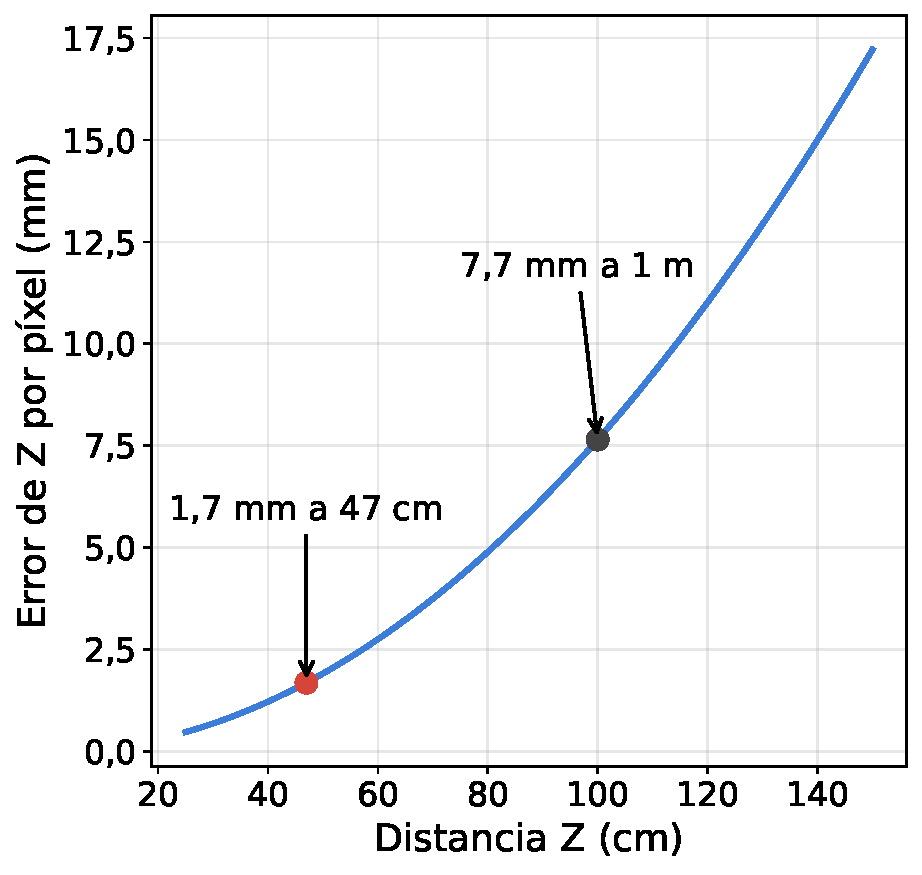
\includegraphics[width=0.8\columnwidth]{fig8_resolucion.pdf}
\caption{Resolución teórica en profundidad por píxel de error en la disparidad para $f=1605{,}9$~px y $B=8{,}14$~cm.}
\label{fig:resolucion}
\end{figure}

% =====================================================================
\section{Conclusiones}
Se desarrolló un sistema que, con dos cámaras web y una red de segmentación de instancias, localiza tomates en 3D con un error del orden del centímetro a medio metro, accesible desde una interfaz web con calibración integrada. Los principales hallazgos son:
\begin{itemize}
\item La tasa de aprendizaje influyó más que el tamaño del modelo: pasar de 0,002 a 0,0005 mejoró el recall y la estabilidad sin costo, mientras que duplicar los parámetros sumó menos de un punto de mAP50-95 y multiplicó por 2,7 el tiempo de inferencia. M3 es el más preciso integrando todos los umbrales; M2 tiene el mejor F1 en el umbral de operación y es la alternativa si se prioriza la velocidad (9,5~ms).
\item La máscara es la clave de la profundidad: la disparidad entre centroides es estable a 0,2~mm entre capturas y no depende de la textura de la piel, donde SGBM falla.
\item Frente al detector clásico, YOLO generaliza mejor, detecta frutos semimaduros y segmenta el fruto completo; OpenCV es 14 veces más rápido en CPU, pero depende de la iluminación y sobresegmenta frutos alargados.
\item Los datos pesaron más que la arquitectura: unir maduros y semimaduros resolvió el problema de la luz cálida mejor que un cambio de modelo, a costa de una mayor sensibilidad a objetos anaranjados.
\end{itemize}

\emph{Limitaciones.} El modelo se entrenó solo con fotografías de invernadero, por lo que es sensible al cambio de dominio (falso positivo con muebles de madera). Persiste un offset sistemático de profundidad de $\sim$1~cm, la validación de localización se realizó con un solo tomate y pocas distancias, las cámaras no están sincronizadas por hardware y la inferencia remota en Colab añade latencia. Las diferencias de métricas entre modelos son pequeñas y no se repitieron con varias semillas.

\emph{Trabajos futuros.} Se propone (i) ajustar el modelo con 100--200 imágenes propias del entorno, etiquetadas de forma semiautomática; (ii) incorporar la corrección del offset del centro óptico en la calibración y validar con más distancias y frutos; (iii) filtrar detecciones fuera del rango de trabajo (0,25--1~m); (iv) exportar el modelo a ONNX/TensorRT para ejecutarlo localmente y usar cámaras sincronizadas; (v) enviar $(X,Y,Z)$ al controlador del brazo para cerrar el ciclo de cosecha; y (vi) volver a distinguir el grado de madurez cuando se disponga de datos con distintas iluminaciones.

% =====================================================================
\begin{thebibliography}{16}

\bibitem{kootstra2021}
G.~Kootstra, X.~Wang, P.~M. Blok, J.~Hemming, and E.~van Henten, ``Selective harvesting robotics: Current research, trends, and future directions,'' \emph{Curr. Robot. Rep.}, vol.~2, no.~1, pp.~95--104, 2021.

\bibitem{rajendran2024}
V.~Rajendran~S., B.~Debnath, S.~Mghames, W.~Mandil, S.~Parsa, S.~Parsons, and A.~Ghalamzan-E., ``Towards autonomous selective harvesting: A review of robot perception, robot design, motion planning and control,'' \emph{J. Field Robot.}, vol.~41, no.~7, 2024.

\bibitem{redmon2016}
J.~Redmon, S.~Divvala, R.~Girshick, and A.~Farhadi, ``You only look once: Unified, real-time object detection,'' in \emph{Proc. IEEE Conf. Comput. Vis. Pattern Recognit. (CVPR)}, 2016, pp.~779--788.

\bibitem{he2017}
K.~He, G.~Gkioxari, P.~Dollár, and R.~Girshick, ``Mask R-CNN,'' in \emph{Proc. IEEE Int. Conf. Comput. Vis. (ICCV)}, 2017, pp.~2961--2969.

\bibitem{zheng2023}
S.~Zheng, Y.~Liu, W.~Weng, X.~Jia, S.~Yu, and Z.~Wu, ``Tomato recognition and localization method based on improved YOLOv5n-seg model and binocular stereo vision,'' \emph{Agronomy}, vol.~13, no.~9, p.~2339, 2023.

\bibitem{zhao2025}
J.~Zhao, W.~Bao, L.~Mo, Z.~Li, Y.~Liu, and J.~Du, ``Design of tomato picking robot detection and localization system based on deep learning neural networks algorithm of Yolov5,'' \emph{Sci. Rep.}, vol.~15, art.~6180, 2025.

\bibitem{hirschmuller2008}
H.~Hirschmüller, ``Stereo processing by semiglobal matching and mutual information,'' \emph{IEEE Trans. Pattern Anal. Mach. Intell.}, vol.~30, no.~2, pp.~328--341, 2008.

\bibitem{yolo11}
G.~Jocher and J.~Qiu, ``Ultralytics YOLO11,'' 2024. [En línea]. Disponible: \url{https://docs.ultralytics.com/models/yolo11/}

\bibitem{laboro}
Laboro.AI, ``Laboro Tomato: Instance segmentation dataset,'' 2020. [En línea]. Disponible: \url{https://github.com/laboroai/LaboroTomato}

\bibitem{feng2021}
C.~Feng, Y.~Zhong, Y.~Gao, M.~R. Scott, and W.~Huang, ``TOOD: Task-aligned one-stage object detection,'' in \emph{Proc. IEEE/CVF Int. Conf. Comput. Vis. (ICCV)}, 2021, pp.~3490--3499.

\bibitem{zhang2000}
Z.~Zhang, ``A flexible new technique for camera calibration,'' \emph{IEEE Trans. Pattern Anal. Mach. Intell.}, vol.~22, no.~11, pp.~1330--1334, 2000.

\bibitem{bradski2008}
G.~Bradski and A.~Kaehler, \emph{Learning OpenCV: Computer Vision with the OpenCV Library}. Sebastopol, CA, USA: O'Reilly, 2008.

\bibitem{li2020}
X.~Li, W.~Wang, L.~Wu, S.~Chen, X.~Hu, J.~Li, J.~Tang, and J.~Yang, ``Generalized focal loss: Learning qualified and distributed bounding boxes for dense object detection,'' in \emph{Adv. Neural Inf. Process. Syst. (NeurIPS)}, vol.~33, 2020, pp.~21002--21012.

\bibitem{bolya2019}
D.~Bolya, C.~Zhou, F.~Xiao, and Y.~J. Lee, ``YOLACT: Real-time instance segmentation,'' in \emph{Proc. IEEE/CVF Int. Conf. Comput. Vis. (ICCV)}, 2019, pp.~9157--9166.

\bibitem{lin2014}
T.-Y. Lin \emph{et al.}, ``Microsoft COCO: Common objects in context,'' in \emph{Proc. Eur. Conf. Comput. Vis. (ECCV)}, 2014, pp.~740--755.

\bibitem{loshchilov2019}
I.~Loshchilov and F.~Hutter, ``Decoupled weight decay regularization,'' in \emph{Proc. Int. Conf. Learn. Represent. (ICLR)}, 2019.

\end{thebibliography}

\end{document}
